\documentclass[12pt]{exam}

\newcommand{\course}{MTH 234 Summer 2021}
\newcommand{\qdate}{15.10} %PUT DATE HERE
\newcommand{\quiz}{Group Work} 

    \usepackage[top=1in, bottom=1in, left=.45in, right=.45in]{geometry}
    \usepackage{amsmath,amsthm,amssymb,amstext}
    \usepackage{enumerate,enumitem}
    \usepackage{tikz,float,graphicx}
    \usepackage{microtype}
    \usepackage{bm,tikz}
        \usetikzlibrary{calc}
    \usepackage{multicol}
    \usepackage{nicematrix}
    \usepackage{cleveref}
    \usepackage[framemethod=tikz]{mdframed}
    
    %\newcommand{\course}{MTH 234 Summer 2021}
    %\newcommand{\qdate}{Equations of lines and planes} %PUT DATE HERE
    %\newcommand{\quiz}{Group Work} 
    
    \newcommand{\R}{\mathbb{R}}
    
    \newcommand{\ba}{\bm{a}}
    \newcommand{\bb}{\bm{b}}
    \newcommand{\bc}{\bm{c}}
    \newcommand{\bi}{\bm{i}}
    \newcommand{\bj}{\bm{j}}
    \newcommand{\bk}{\bm{k}}
    \newcommand{\br}{\bm{r}}
    \newcommand{\bv}{\bm{v}}
    \newcommand{\gen}[1]{\left\langle #1 \right\rangle}

\newtheorem*{theorem}{Theorem}
\surroundwithmdframed[]{theorem}

\theoremstyle{definition}
    \newtheorem*{definition}{Definition}
    \surroundwithmdframed[]{definition}
    \newtheorem*{info}{Useful Information}
    \surroundwithmdframed[]{info}
\theoremstyle{remark}
    \newtheorem*{remark}{Remark}
    \surroundwithmdframed[]{remark}
    

%%%%%%%%%%%%%%%%%%%%%%%
% HEADER AND FOOTER
%%%%%%%%%%%%%%%%%%%%%%%
\pagestyle{headandfoot}
\firstpageheadrule
\runningheadrule
\firstpageheader{\course}{\quiz}{\qdate}
\runningheader{\course}{\quiz}{\qdate}
\runningfooter{}{}{}


\usepackage{color}
\shadedsolutions
\definecolor{SolutionColor}{rgb}{0.8,0.9,1}

\usepackage{pgfplots}
    \pgfplotsset{every axis/.append style={
                    axis x line=middle,    % put the x axis in the middle
                    axis y line=middle,    % put the y axis in the middle
                    axis line style={<->}, % arrows on the axis
                    xlabel={$x$},          % default put x on x-axis
                    ylabel={$y$},          % default put y on y-axis
                    grid=both,
                    %xtick={-4,...,-1,1,...,3},
                    %ytick={-1,1,}
    }}
    \pgfplotsset{compat=1.17}

\newcommand{\bif}{\quad\iff\quad}
\usetikzlibrary{patterns}

\printanswers
%\noprintanswers

\begin{document}

\section*{\qdate}

%\subsection*{Template}

\begin{info}
    \begin{itemize}
            \item The \textbf{Jacobian} for a tranformation \(T\) given by \(x=x(u,v)\) and \(y=y(u,v)\) is
            \[
                \dfrac{(x,y)}{(x,y)}=
                \left|\begin{NiceMatrix}
                    \pd{x}{u} & \pd{x}{v}\\
                        &\\
                    \pd{y}{u} & \pd{y}{v}
                \end{NiceMatrix}\right| = \pd{x}{u}\cdot\pd{y}{v}-\pd{x}{v}\cdot\pd{y}{u}
            \]
            \item 
            \[
                \iint_{R}f(x,y)~dA=\iint_{S}f(x(u,v),y(u,v))\left|\dfrac{(u,v)}{(u,v)}\right|~du~dv
            \]
    \end{itemize}
\end{info}


\begin{questions}

\question Let \(S\) be the square \(\{(u,v)~:~0\le u \le 1,0\le v\le 1\}\) and let \(T\) be the transformation
    \[
        x=v,~y=u(1+v^2)
    \]
\begin{parts}
    \part Let \(L_1\),\(L_2\),\(L_3\), and \(L_4\) denote the left, bottom, right, and top sides of \(S\) respectively.

    \(L_1\) is the line \(u=0\) and \(0\le v\le 1\). So on \(L_1\), \(x=v\) and \(y=0\) with

    \[L_1:~~~~ y=0,\quad \text{with} 0\le x\le 1\]

    Express the image of \(L_2\), \(L_3\), and \(L_4\) similarly.

        \ifprintanswers
        \begin{solution}
            Along \(L2\) \(v=0\) and \(0\le u \le 1\), which gives
                \[
                    x=0, ~~0\le y\le 1
                \]
                Similiarly 
                \begin{equation*}
                    \begin{aligned}
                        L3: ~~~~y&=1+x^2 & 0\le x \le 1\\
                        L4:~~~~x & =1 & 0\le y\le 2
                    \end{aligned}
                \end{equation*}

        \end{solution}
    \else
        \vfill
    \fi

    \part Sketch the image of \(S\) under the transformation given.
        \ifprintanswers
        \begin{solution}
            \begin{center}
            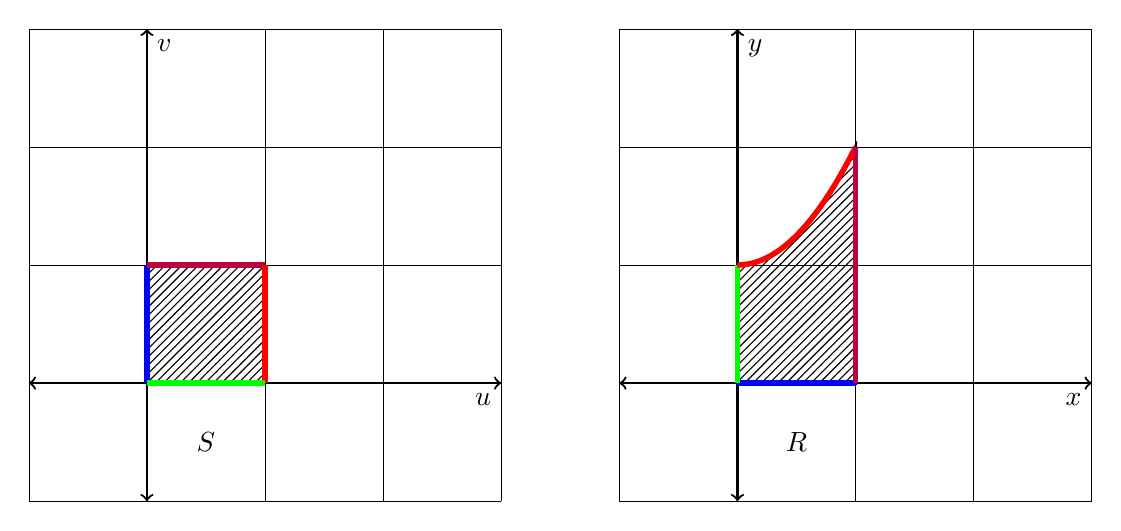
\begin{tikzpicture}[scale=1.5]
                \begin{scope}
                \draw[fill=white,white] (-1,-1)--(3,-1)--(3,3)--(-1,3)--(-1,-1);
                    \draw[very thin] (-1,-1) grid (3,3);
                    \draw[<->,thick] (-1,0)--(3,0) node[anchor=north east] {$u$};
                    \draw[<->,thick] (0,-1)--(0,3) node[anchor=north west] {$v$};
                    \draw[fill=white] (0,0)--(1,0)--(1,1)--(0,1)--(0,0);
                    \draw[thin, pattern=north east lines] (0,0)--(1,0)--(1,1)--(0,1)--(0,0);

                    \draw[line width=2pt,blue] (0,0)--(0,1);
                    \draw[purple,line width=2pt] (0,1)--(1,1);
                    \draw[red,line width=2pt] (1,0)--(1,1);
                    \draw[green,line width=2pt] (0,0)--(1,0);
                    \node at (.5,-.5) {$S$};
                \end{scope}

                \begin{scope}[shift={(5,0)}]
                \draw[fill=white,white] (-1,-1)--(3,-1)--(3,3)--(-1,3)--(-1,-1);
                    \draw[very thin] (-1,-1) grid (3,3);
                    \draw[<->,thick] (-1,0)--(3,0) node[anchor=north east] {$x$};
                    \draw[<->,thick] (0,-1)--(0,3) node[anchor=north west] {$y$};
                    \draw[very thick,pattern=north east lines,domain=0:1,smooth,variable=\x] plot ({\x},{1+\x*\x}) --(1,0)--(0,0)--(0,1);
                    
                    \draw[blue,line width=2pt] (0,0)--(1,0);
                    \draw[green,line width=2pt] (0,0)--(0,1);
                    \draw[red,line width=2pt,domain=0:1,smooth,variable=\x] plot ({\x},{1+\x*\x});
                    \draw[purple,line width=2pt] (1,0)--(1,2);
                    \node at (.5,-.5) {$R$};
                \end{scope}
            \end{tikzpicture}
            \end{center}
        \end{solution}
    \else
        \vfill
    \fi
    \end{parts}

\question Repeat the above instructions for \(S\) the triangular region of the \(uv\)-plane with vertices \((0,0)\), \((1,1)\), and \((0,1)\) with the transformation
\[
        x=u^2,y=v.
\]
\ifprintanswers
        \begin{solution}
            The lines bounding \(S\) are
            \begin{align*}
                L1:~~~~ u&=0 ~~~~\Longrightarrow~~~~ x=0,~~0\le y \le 1\\
                L2:~~~~ v&=1 ~~~~\Longrightarrow~~~~ y=1,~~0\le x \le 1\\
                L3:~~~~ v&=u ~~~~\Longrightarrow~~~~ x=y^2,~~0\le y \le 1\\
            \end{align*}
            \begin{center}
            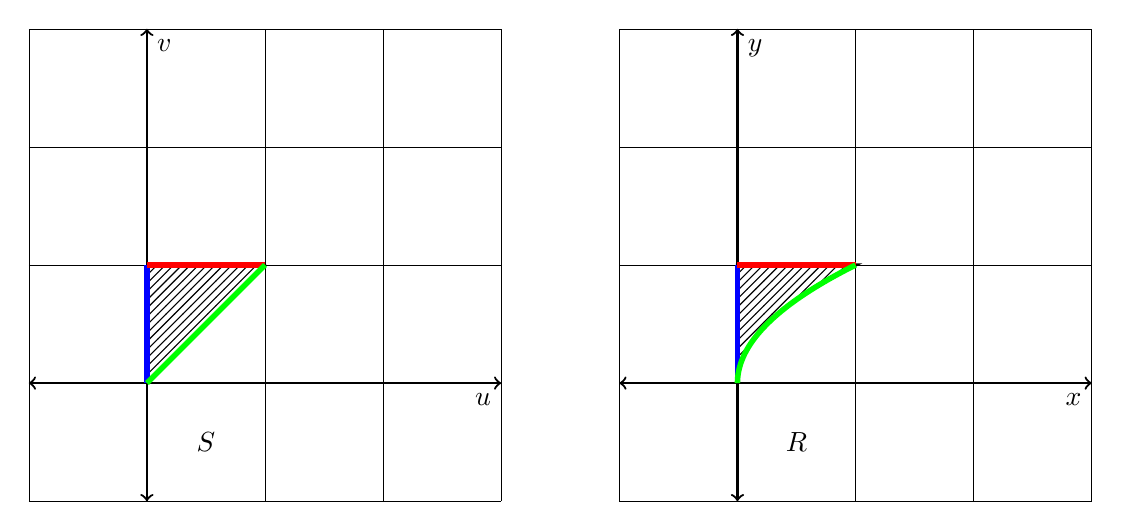
\begin{tikzpicture}[scale=1.5]
                \begin{scope}
                \draw[fill=white,white] (-1,-1)--(3,-1)--(3,3)--(-1,3)--(-1,-1);
                    \draw[very thin] (-1,-1) grid (3,3);
                    \draw[<->,thick] (-1,0)--(3,0) node[anchor=north east] {$u$};
                    \draw[<->,thick] (0,-1)--(0,3) node[anchor=north west] {$v$};
                    \draw[thin, pattern=north east lines] (0,0)--(0,1)--(1,1)--(0,0);

                    \draw[line width=2pt,blue] (0,0)--(0,1);
                    \draw[red,line width=2pt] (0,1)--(1,1);
                    \draw[green,line width=2pt] (0,0)--(1,1);
                    \node at (.5,-.5) {$S$};
                \end{scope}

                \begin{scope}[shift={(5,0)}]
                \draw[fill=white,white] (-1,-1)--(3,-1)--(3,3)--(-1,3)--(-1,-1);
                    \draw[very thin] (-1,-1) grid (3,3);
                    \draw[<->,thick] (-1,0)--(3,0) node[anchor=north east] {$x$};
                    \draw[<->,thick] (0,-1)--(0,3) node[anchor=north west] {$y$};
                    \draw[very thick,pattern=north east lines,domain=0:1,smooth,variable=\x] plot ({\x*\x},{\x}) --(0,1)--(0,0);
                    
                    \draw[line width=2pt,blue] (0,0)--(0,1);
                    \draw[line width=2pt,red] (0,1)--(1,1);
                    \draw[green,line width=2pt,domain=0:1,smooth,variable=\x] plot ({\x*\x},{\x});
                    \node at (.5,-.5) {$R$};
                \end{scope}
            \end{tikzpicture}
            \end{center}

        \end{solution}
    \else
        \vfill
    \fi

\newpage

\question Let \(R\) be the parallelogram with vertices \((0,0), (4,3), (2,4), (-2,1)\). Let \(S\) be the square \([0,1]\times[0,1]\). Find a transformation that maps \(S\) onto \(R\).

Suggestion: Experiment and try stuff. What points in \(S\) are sent to the corners of \(R\)?
\ifprintanswers
        \begin{solution}
            \[
            x=4u-2v,~~~~y=3u+v
            \]
        \end{solution}
    \else
        \vfill
    \fi 

\question Evaluate the integral 
\[
        \iint_R e^{(x+y)/(x-y)}~dA
\]
where \(R\) is the trapezoidal region with vertices \((1,0), (2,0), (0,-2), (0,-1)\).
\begin{parts}
    \part Since this is not easy as written, we want to do a change of variables. Based on the given function, we will try
    \[
        u=x+y,\quad v=x-y.
    \]
    Then we want to use the transformation \(T\) given by \(x=\frac{1}{2}(u+v)\) and \(y=\)?
    \ifprintanswers
        \begin{solution}
            Solve for \(y\) by using the above and \(u-v=(x+y)-(x-y)=2y\) to get
            \[
                y=\frac{1}{2}(u-v).
            \]
        \end{solution}
    \else
        \vfill
    \fi

    \part Setting \(u=x+y\) and \(v=x-y\), what is the image of the trapezoidal region given?
    \ifprintanswers
        \begin{solution}
            \[
            \begin{array}{ c | c }
               (x,y) & (u,v)\\ \hline 
                (1,0) & (1,1)\\
                (2,0) & (2,2)\\
                (0,-2) & (-2,2)\\
                (0,-1) & (-1,1)\\
            \end{array}
            \]
            With $S$ the region
            \begin{center}
            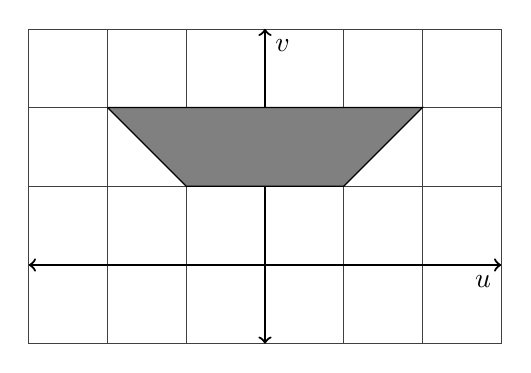
\begin{tikzpicture}
                \draw[fill=white,white] (-3,-1) rectangle (3,3);
                \draw[very thin,opacity=.75] (-3,-1) grid[step=1] (3,3);
                    \draw[<->,thick] (-3,0)--(3,0) node[anchor=north east] {$u$};
                    \draw[<->,thick] (0,-1)--(0,3) node[anchor=north west] {$v$};
                    \draw[fill=gray] (-2,2)--(-1,1)--(1,1)--(2,2)--(-2,2);
                \end{tikzpicture}
            \end{center}
        \end{solution}
    \else
        \vfill
    \fi

    \part Evaluate the integral.
    \ifprintanswers
        \begin{solution}
            \begin{align*}
                \iint_R e^{(x+y)/(x-y)}~dA & = \iint_S e^{u/v}\pd{(x,y)}{(u,v)}~dA\\
                    & = \iint_S e^{u/v} \left( \left(\frac{1}{2}\right)\left(\frac{1}{2}\right)-\left(\frac{1}{2}\right)\left(-\frac{1}{2}\right) \right) ~dA\\
                    & = \frac{1}{2} \int_{1}^2\int_{-v}^{v}e^{u/v}~du~dv\\
                    & = \frac{1}{2} \int_1^2 \left(v(e^{v/v}-e^{-v/v})\right)~dv\\
                    &= \frac{e-e^{-1}}{2} \int_{1}^2 v~dv\\
                    & = \frac{3}{4}\left(e-e^{-1}\right).
            \end{align*}
        \end{solution}
    \else
        \vfill
    \fi
\end{parts}



\newpage


\question Evaluate \(\iint_{R}xy~dA\) where \(R\) is the region in the first quadrant bounded by
\[
    y=x,\quad y=3x,\quad xy=1, \quad xy=3.
\]
using the transformation \(x=u/v,y=v\).


\begin{parts}
    \part Complete the following, determining the image of each line or curve:
    \begin{itemize}
        \item
            \[
                y=x\quad \mapsto \quad v^2=u \text{~~or~~} v=\pm\sqrt{u}
            \]
        \item 
            \[
                y=3x \quad \mapsto \quad  
            \]
        \ifprintanswers
            \begin{solution}
            \[
            v=3u/v\quad\Rightarrow\quad \frac{1}{3}v^2=u \text{~~or~~} v=\pm\sqrt{3u}
            \]     
            \end{solution}
        \else
        \fi
        \item 
            \[
                xy=1 \quad \mapsto \quad  u=1
            \]    
        \item 
            \[
                xy=3 \quad \mapsto \quad  
            \]
        \ifprintanswers
            \begin{solution}
                \[
                    \frac{u}{v}\cdot v = 3 \quad\Rightarrow\quad u=3
                \]
            \end{solution}
        \else
        \fi
\end{itemize}
        \part Rewrite the original double integral using the given transformation
        
        \[
            \int_{a}^b\int_{c}^d f(u,v)~dv~du
        \]
        What are the values of \(a,b,c,d\) and \(f(u,v)\)?
        \ifprintanswers
        \begin{solution}
        
        After the transformation we are integrating over the region bounded by the lines above, as seen below:

            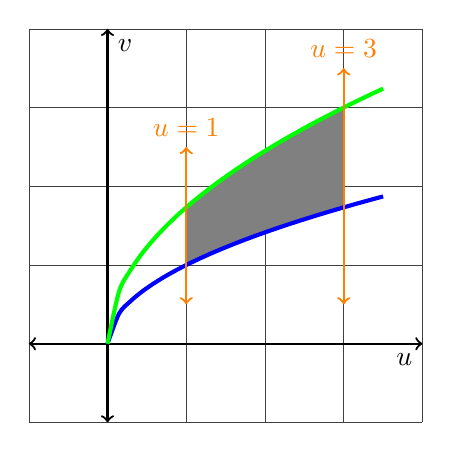
\begin{tikzpicture}%[x=.75cm,y=.75cm]
                \draw[fill=white,white] (-1,-1) rectangle (4,4);
                \draw[very thin,opacity=.75] (-1,-1) grid[step=1] (4,4);
                    \draw[<->,thick] (-1,0)--(4,0) node[anchor=north east] {$u$};
                    \draw[<->,thick] (0,-1)--(0,4) node[anchor=north west] {$v$};

                    \draw[fill=gray,gray] (1,1)--({1},{sqrt(3)}) plot[smooth,domain=1:3,variable=\x] ({\x},{sqrt(3)*sqrt(\x)}) -- ({3},{sqrt(3)});
                    \draw[fill=gray,gray] plot[smooth,domain=1:3,variable=\x] ({\x},{sqrt(\x)}) -- ({3},{sqrt(3)}) -- ({1},{sqrt(3)}) --(1,1);
                    
                    \draw[blue,line width=1.5pt,domain=0:3.5,smooth,variable=\x] plot ({\x},{sqrt(\x)});
                    \draw[green,line width=1.5pt,domain=0:3.5,smooth,variable=\x] plot ({\x},{sqrt(3)*sqrt(\x)});
                    
                    \draw[orange,thick,<->] (1,.5)--(1,2.5) node[above] {$u=1$};
                    \draw[orange,thick,<->] (3,.5)--(3,3.5) node[above] {$u=3$};
            \end{tikzpicture}

        Since 
        \[
            \pd{(x,y)}{(u,v)} = \pd{x}{u}\cdot\pd{y}{v}-\pd{x}{v}\cdot\pd{y}{u} = \left(\dfrac{1}{v}\right)\left(1\right)-\left(0\right) = \dfrac{1}{v},
        \]
        the integral is 
        \begin{align*}
            \iint_{R}xy~dA & = \iint_S \left(\frac{u}{v}\right)\left(v\right)\left(\pd{(x,y)}{(u,v)}\right)~dA\\
                &= \int_1^3\int_{\sqrt{u}}^{\sqrt{3u}} \dfrac{u}{v}~dv~du\\
        \end{align*}
        \end{solution}
    \else
        \vfill
    \fi

        \part Evaluate the integral.
        \ifprintanswers
        \begin{solution}
        From above,
        \begin{align*}
            \int_1^3\int_{\sqrt{u}}^{\sqrt{3u}} \dfrac{u}{v}~dv~du & = \int_1^3 u\left(\ln(v)|_{\sqrt{u}}^{\sqrt{3u}}\right)~du\\
                &= \int_{1}^{3} u\left(\ln(\sqrt{3u})-\ln(\sqrt{u})\right)~du\\
                &= \int_1^3 u\left(\frac{1}{2}\ln(3)+\frac{1}{2}\ln(u)-\frac{1}{2}\ln(u)\right)~du\\
                &= \frac{\ln(3)}{2}\left(\int_{1}^3 u ~du\right)\\
                &= \frac{\ln(3)}{2}\left(\frac{9}{2}-\frac{1}{2}\right)\\
                &= 2\ln(3).
        \end{align*}
        \end{solution}
    \else
        \vfill
    \fi

\end{parts}


\end{questions}

\end{document}

% soln : Question environment
    \ifprintanswers
        \begin{solution}
        \end{solution}
    \else
        \vfill
    \fi